\documentclass[article,A4,12pt]{llncs}
\usepackage[T1]{fontenc}
\usepackage{amsmath}
\usepackage{amssymb}
\usepackage{amsfonts}
\usepackage{mathrsfs, bm}

\usepackage{graphicx}
\usepackage{tabularx}
\usepackage{subfig}
\usepackage{epsf,times}
\usepackage{color}
\usepackage{wrapfig}
\usepackage{cases}
\usepackage{multicol}

\usepackage[T1]{fontenc}
%\newcommand{\tmname}[1]{\textsc{#1}}
%\newcommand{\tmop}[1]{\ensuremath{\operatorname{#1}}}
%\newcommand{\tmsamp}[1]{\textsf{#1}}
%\newcommand{\tmtextsc}[1]{{\scshape{#1}}}
%\newcommand{\tmtextsl}[1]{{\slshape{#1}}}
%\newcommand{\tmtexttt}[1]{{\ttfamily{#1}}}

\leftmargin=0.0cm
\oddsidemargin=0.5cm
\evensidemargin=0.5cm
\topmargin=0cm
\textwidth=16.0cm
%\textheight=21.5cm
\textheight=20.0cm
\pagestyle{plain}
\setlength{\columnsep}{20pt}

\def\m{\mathbf{m}}
\def\H{\mathbf{H}}
\def\E{\mathbf{E}}
\newcommand{\vepsi}{{\varepsilon}}
\def\hnorm#1#2{\vert\,#1\,\vert_{#2}}
\newcommand{\R}{{\mathbb R}}
\newcommand{\Sph}{{\mathbb S}}
\def\x{\mathbf{x}}
\def\hvec{\overline{\mathbf{h}}}
\def\evec{\overline{\mathbf{e}}}

\newcommand{ \etal}{\mbox{\emph{et al. }}}

\newcommand\vect[1]{\mbf{#1}}
\newcommand{\mbf}[1]{\mbox{\boldmath$#1$}} 
\newcommand{\RC}[1]{#1 $\times$ #1 $\times$ #1}
\def\um{$\mu$m}
\def\C{$^{\circ}\mathrm{C}$}

\newcommand{\Rmnum}[1]{\expandafter\@slowromancap\romannumeral #1@}

% DEFINITION OF CUSTOM FONT SIZE
\newcommand{\customfontA}{\fontsize{50}{55}\selectfont}
\newcommand{\customfontB}{\fontsize{14.4}{20}\selectfont}
\newcommand{\customfontC}{\fontsize{30}{35}\selectfont}

\DeclareMathAlphabet{\mathpzc}{OT1}{pzc}{m}{it}

\def\clovek#1{\noindent\bgroup\vbox{\noindent#1}\egroup\vskip1em}

% TO INPUT BACKGROUND IMAGE
\usepackage{eso-pic}
\newcommand\BackgroundPic{
\put(0,0){
\parbox[b][\paperheight]{\paperwidth}{
\vfill
\centering
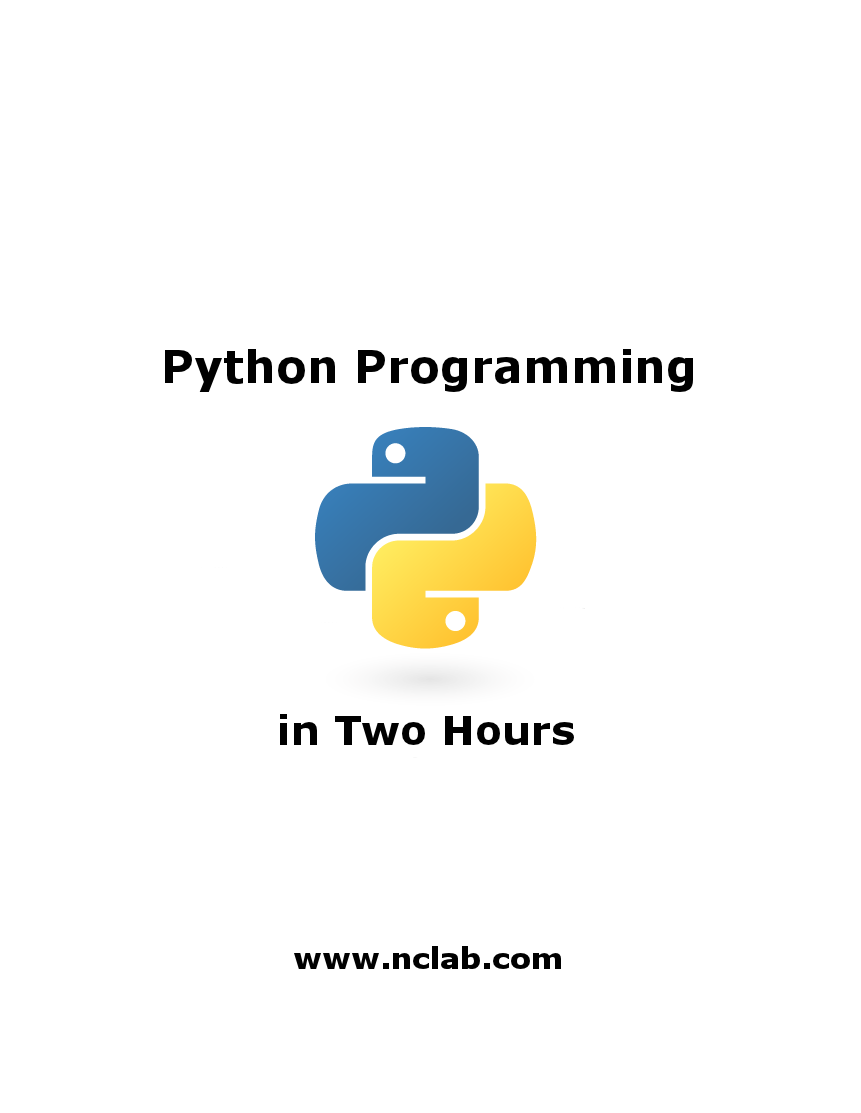
\includegraphics[width=\paperwidth,height=\paperheight]{img/python-frontpage.png}
%\includegraphics[width=\paperwidth,height=\paperheight]{img/background.jpg}
\vfill
}}}

\begin{document}

% INPUTTING BACKGROUND IMAGE
\AddToShipoutPicture{\BackgroundPic}
\vbox{}
\pagestyle{empty}
\newpage
\textwidth=15.5cm
\ClearShipoutPicture
\newpage

%%%%%%%%%%%%%%%%%%%%%%%%%%%%%%%%%%%%%%%%%%%%%%%%%%%%%%%%%%%%%%%%%%%%%%%%%

\section*{}
\small
\subsection*{About NCLab}
Networked Computing Laboratory (NCLab) is a popular Internet-based framework for 
programming, mathematics, computer modeling, 
and scientific computing. It serves students, instructors, researchers, and the general 
public. NCLab can be used free of charge for personal non-commercial purposes such as 
private hobby or self-education, as well as for individual non-funded academic research.
All other use is subject to {\bf purchasing a license} for a symbolic fee. The fees are as low as 
\$1 per user per month for educational use, and they are used to support the development 
and operational expenses. NCLab is a product of FEMhub Inc. The name "NCLab" is 
registered with the U.S. Patent and Trademark Office (USPTO) under Trademark No. 85420518.

\subsection*{Terms of Use and Pricing}
More details on purchasing a license and using NCLab are provided in the online documents 
{\bf Pricing} and {\bf Terms of Use} that are accessible from NCLab's home page 
{\tt http://nclab.com}.

\subsection*{Contact Information}
General inquiries: {\tt info@femhub.com}\\
Sales: {\tt sales@femhub.com}\\
NCLab support: {\tt support@nclab.com}\\
Agros \& Hermes support: {\tt support@femhub.com}\\
Web page: {\tt http://femhub.com}\\
{Physical address}\\
FEMhub Inc.\\
5490 Twin Creeks Dr.\\
Reno, NV 89523

\subsection*{About This Publication}
This publication can be copied and distributed without any restrictions
as long as reference to NCLab and FEMhub Inc. is preserved.

\subsection*{Acknowledgement}
This publication was created with the help of numerous freely 
available web resources and tutorials related to Python, in
particular the Python Tutorial at www.python.org.

\normalsize

\newpage
%{\ }
\setcounter{tocdepth}{2}
\tableofcontents
%\pagestyle{plain}

\newpage

\pagestyle{plain}
\setcounter{page}{1}

%%%%%%%%%%%%%%%%%%%%%%%%%%%%%%%%%%%%%%%%%%%%%%%%%%%%%%%%%%%%%%%%%%%%%%%%%

\section{Introduction}

Python is an easy to learn, powerful programming language. It has efficient high-level 
data structures and a simple but effective approach to object-oriented programming. 
Python's elegant syntax and dynamic typing, together with its interpreted nature, 
make it an ideal language for scripting and rapid application development in many 
areas on most platforms. 

Python is an interpreted language, which can save you considerable time during program 
development because no compilation and linking is necessary. The interpreter can be used 
interactively, which makes it easy to experiment with features of the language, to write 
throw-away programs, or to test functions during bottom-up program development. It is also 
a handy desk calculator.

In this tutorial we introduce various features of the Python language and system through examples, 
beginning with simple expressions, statements and data types, through functions and modules, 
and finally touching upon advanced concepts like exceptions and user-defined classes.



\section{Numbers}



\section{Strings}



\section{Lists}



\section{Conditions}



\section{The {\tt for} loop}



\section{The {\tt range()} function}



\section{The {\tt break} and {\tt continue} statements}



\section{The {\tt else} clause for loops}



\section{The {\tt pass} statement}




\section{Defining new functions}


\subsection{Default argument values}


\subsection{Keyword arguments}


\subsection{Arbitrary argument lists}


\subsection{Unpacking argument lists}


\subsection{Lambda forms}


\subsection{Documentation strings}


\section{More on lists}


\subsection{Using lists as stacks}


\subsection{Using lists as queues}


\subsection{Functional programming tools}


\subsection{List comprehensions}


\section{The {\tt del} statement}


\section{Tuples and sequences}


\section{Sets}


\section{Dictionaries}


\section{Looping techniques}


\section{Input and output}


\section{Errors and Exceptions}


\subsection{Syntax errors}


\subsection{Exceptions}


\subsection{Handling exceptions}


\subsection{Raising exceptions}


\subsection{User-defined exceptions}


\subsection{Defining clean-up actions}


\section{Classes}


\subsection{Inheritance}


\subsection{Private variables}


\subsection{Iterators}


\subsection{Generators}










\end{document}
